\documentclass[a4paper]{article}
\usepackage{fullpage}
\usepackage{hyperref}
\usepackage{graphicx}
\title{Scenario Editor}
%\author{Group 3 of the A Search And Rescue Context Project}
\date{}
\begin{document}
\maketitle
\newpage

\tableofcontents
\newpage

\section{Introduction}
This document describes how to make use of the Scenario Editor. When you open the editor, you see two main parts:
\begin{enumerate}
\item The Configuration panel, which is used to create, open and save configuration files.
\item The Bot panel, where a list of the bots is being displayed. Here you can create, modify, rename, duplicate and delete bots. At the top of this panel is indicated how many bots, e-partners and humans are currently created.
\end{enumerate}

\begin{figure}
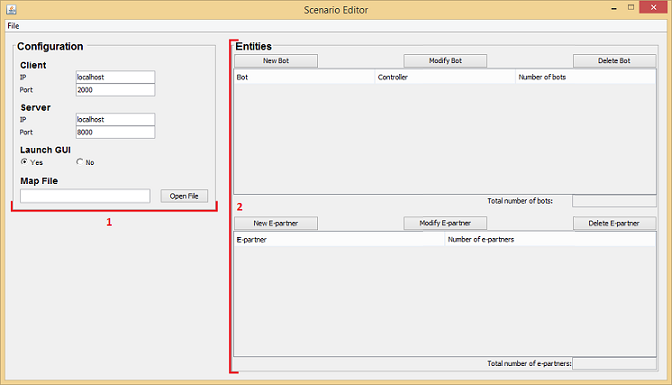
\includegraphics{editor.png}
\end{figure}

\section{General use}
At the top of the editor you can see a $File$ menu. If you click on that, you get the options to create a new configuration, save your configuration, open a configuration and to exit the editor.

On the left side of the editor you can configure a scenario as you like. The Client IP, the Client Port, the Server IP and the Server Port should already contain the default values. You can change them if you need to. You can also indicate whether you want to make use of GOAL and/or open a GUI. If you have an Agent class file or a Map file you want to use, you can import them by selecting the $Open$ $file$ buttons at the right sections.

On the right side of the editor you can create, modify, rename, duplicate and delete bots. There also is a list of bots that are created, and on top of the list there is an indication of how many bots, e-partners and humans there are.
\pagebreak
\section{Configuration Panel}
\begin{figure}
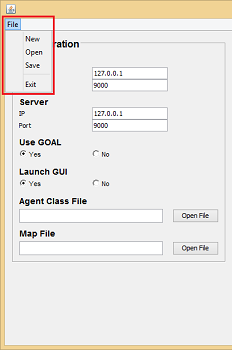
\includegraphics{config.png}
\end{figure}
\subsection{New configuration file}
To create a new configuration file, select $File$ $\to$ $New$ in the menu bar at the top of the editor. You will now get a new configuration with the default values. Creating a new configuration will reset all previous changes you have made, so make sure you save your configuration first if you want to want to keep it.

\subsection{Save configuration file}
To save your configuration file, select $File$ $\to$ $Save$ in the menu bar at the top of the editor. A screen will pop up where you can select the folder you want to save the file to. Once you have selected the right folder, click the $Save$ button.

\subsection{Open configuration file}
To open an existing configuration file, select $File$ $\to$ $Open$ in the menu bar at the top of the editor. A screen will pop up where you can select the folder where the configuration file is saved to. Once you have selected the right folder, select the file and click the $Open$ button.
\pagebreak
\section{Bot Panel}
\begin{figure}
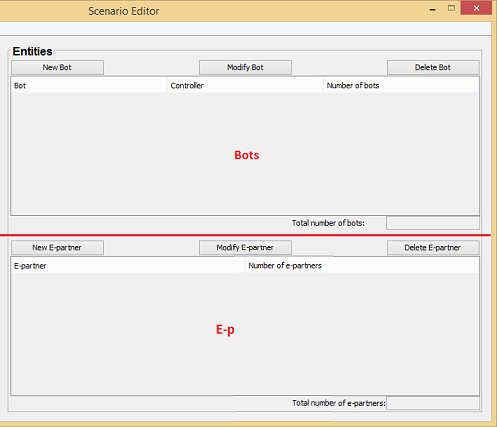
\includegraphics{bot.png}
\end{figure}
\subsection{Create new bot}
To create a new bot, click the $New$ $bot$ button at the right side of the editor. The Bot Store will open in a new window where you can create your bot.

\subsection{Modify bot}
To modify a bot, select the bot you want to modify in the bot list and click the $Modify$ $bot$ button at the right side of the editor. The bot store will open in a new window where you can modify your bot.

\subsection{Rename bot}
To rename a bot, select the bot you want to rename in the list with bots. Enter the new name in the textfield above the $Rename$ $bot$ button at the right side of the editor and click the $Rename$ $bot$ button.

\subsection{Duplicate bot}
To duplicate a bot, select the bot you want to duplicate in the list with bots. Enter the number of times you want to duplicate the bot in the box above the $Duplicate$ $bot$ button at the right side of the editor and click the $Duplicate$ $bot$ button.

\subsection{Delete bot}
To delete a bot, select the bot you want to delete in the list with bots and click the $Delete$ $bot$ button at the right side of the editor.
\end{document}